\documentclass[../main.tex]{subfiles}

\begin{document}

\section{Tree-level OPEs}

In this section we initiate our computation of OPEs of the gravitational side chiral algebra, using the same techniques as in \cite{CPt4}.

\subsection{Explicit expressions for supergravity states}

Recall that the full classical coupling of Kodaira--Spencer theory is
\[
\int_{\C^{3|4}} \mu_1 \mu_2 \mu_z \; \d z \d^2 w \d^4 \eta + \int_{\C^{3|4}} \alpha \mu_i \partial_{w_i} \gamma \; \d z \d^2 w \d^4 \eta + \int_{\C^{3|4}} \alpha \mu_z \partial_z \gamma \; \d z \d^2 w \d^4 \eta .
\]

We will use the notation $D_{r,s}$ to denote the holomorphic differential operator
\[ 
	D_{r,s} = \frac{1}{r!} \frac{1}{s!} \partial_{w_1}^r \partial_{w_2}^s. 
\]  

\subsection{$\til J \til J$ OPE}

We first compute the OPE of the off-shell operators $\til{J}^i[r,s]$ and then impose constraints to determine the OPE of the on-shell operators $J[r,s]$.

The coefficient of $\til{J}^1[k,l]$ in the OPE will be determined by the terms in the BRST variation of $\mu_1$ which involve $\fc_1$ and $\mu_1$, $\fc_1$ and $\mu_2$, or $\fc_2$ and $\mu_1$. 

Consider the gauge variation of 
\begin{equation}\label{eqn:j1vary}
	\int_{(z,\eta_a) \in \C^{1 \mid 4}} \til{J}^1[r,s](z,\eta_a)  D_{r,s} \mu_1(z,w_i = 0,\eta_a) . 
\end{equation}
The gauge variation of $\mu_1$ is
\begin{align*}
	Q \mu_1 & = \dbar \mf{c}_1 + \mu_i \partial_{w_i} \mf{c}_1 + \mu_z \partial_{z} \mf{c}_1 - \mf{c}_i \partial_{w_i} \mu_1 - \mf{c}_z \partial_z \mu_1 \\
& + \partial_{w_2} \fc_\gamma\partial_z \alpha -  \partial_z\fc_\gamma \partial_{w_2} \alpha + \partial_{w_2} \fc_\alpha \partial_z \gamma - \partial_z \fc_\alpha \partial_{w_2} \gamma .
\end{align*}
For now, we can disregard the terms involving $\fc_\gamma$ and $\alpha$ or $\fc_\alpha$ and $\gamma$.
These will play a role later on when we constrain the OPE's involving the operators $G_\alpha, G_\gamma$.

Inserting this gauge variation into the coupling to $\til{J}^i[r,s]$, we see that the first term, $\dbar \mf{c}_1$, vanishes by integration by parts.  
Cancellation of the remaining terms will give us constraints on the OPE coefficients.
The remaining terms are 
\[ 
	\int_{z,\eta_a} \til{J}^1[r,s] (z,\eta_a)  D_{r,s}\left( \mu_i \partial_{w_i} \mf{c}_1 + \mu_z \partial_{z} \mf{c}_1 - \mf{c}_i \partial_{w_i} \mu_1 - \mf{c}_z \partial_z \mu_1 \right)(z,w_i = 0, \eta_a). 
\]
Let us focus on the term in this expression which involves the fields $\mu_1$ and $\mf{c}_1$. This is 
\[ 
	 \int_{z,\eta_a} \til{J}^1[r,s] (z,\eta_a)  D_{r,s}\left( \mu_1 \partial_{w_1} \mf{c}_1   - \mf{c}_1 \partial_{w_1} \mu_1  \right)(z,w_i = 0, \eta_a). 
\]
Because this expression involves both $\mf{c}_1$ and $\mu_1$, which are fields (and a corresponding ghost) that couple to $\til{J}^1$, we find that it can only be cancelled by a gauge variation of an integral involving two copies of the operators $\til{J}^1$, at separate points $z,z'$:  
\[ 
	\tfrac{1}{2} \int_{z,z', \eta_a,\eta_a'} \til{J}^1[k,l] (z,\eta_a) D_{k,l} \mu_1(z, w_i = 0, \eta_a)  \til{J}^1[r,s] (z',\eta'_a) D_{r,s} \mu_1(z', w'_i = 0, \eta'_a) . 
\]
Applying the gauge variation of $\mu_1$ to this expression, and retaining only the terms involving $\dbar \mf{c}_1$, gives us
\[ 
	\int_{z,z', \eta_a,\eta_a'} \til{J}^1[k,l] (z,\eta_a) D_{k,l} \mu_1(z, w_i = 0, \eta_a)  \til{J}^1[r,s] (z',\eta'_a) D_{r,s} \dbar \mf{c}_1 (z', w'_i = 0, \eta'_a) . 
\]
Here the $\dbar$ operator only involves the $z$-component because restricting to $w_i= 0$ sets any $\d \wbar_i$ to zero. We can integrate by parts to move the location of the $\dbar$ operator. Every field $\mu_i$ contains a $\d \zbar$, as otherwise it would restrict to zero at $w_i = 0$, so that $\partial_{\zbar} \mu_i = 0$. 

This discussion shows that in order for the anomaly to cancel we need
\begin{multline} 
	\int_{z,z', \eta_a,\eta_a'} \dbar_{\zbar} \left( \til{J}^1[k,l] (z,\eta_a)  \til{J}^1[r,s] (z',\eta'_a) \right)  D_{m,n} \mu_1(z, w_i = 0, \eta_a)  D_{r,s}  \mf{c}_1 (z', w'_i = 0, \eta'_a)  \\
	= \int_{z'',\eta''_a} \til{J}^1[m,n] (z'',\eta''_a)  D_{m,n}\left( \mu_1 \partial_{w_1} \mf{c}_1   - \mf{c}_1 \partial_{w_1} \mu_1  \right)(z'',w_i = 0, \eta''_a).   
\end{multline}
In these expressions, we sum over the indices $r,s,k,l,m,n$.  This equation must hold for all values of the field $\mu_1$, $\mf{c}_1$. To constrain the OPEs, we can test the equation by setting 
\begin{align*}
\mu_1 & = G(z,\zbar,\eta_a) \d \zbar w_1^k w_2^l \\
\mf{c}_1 & = H(z,\zbar,\eta_a) w_1^r w_2^s
\end{align*}
for $G,H$ arbitrary smooth functions of the variables $z,\zbar,\eta_a$. 

Inserting these values for the fields into the anomaly-cancellation condition gives
\begin{multline} 
	\int_{z,z', \eta_a,\eta_a'} \dbar_{\zbar} \left( \til{J}^1[k,l] (z,\eta_a)  \til{J}^1[r,s] (z',\eta'_a) \right)  G(z,\zbar,\eta_a) H(z',\zbar',\eta_a') \\ 
	= \int_{z'',\eta''_a} (r-k)  \til{J}^1[k+r-1, l+s] (z'',\eta''_a)  G(z'',\zbar'',\eta''_a) H(z'',\zbar'', \eta_a'').
\end{multline}
Since this must hold for all values of the functions $G,H$ we get an identity of the integrands:
\[ 
	\dbar_{\zbar} \left( \til{J}^1[k, l] (z,\eta_a)  \til{J}^1[r,s] (z',\eta'_a) \right)  = \delta_{z = z',\br{z} = \br{z}'} \delta_{\eta_a = \eta'_a} (r-m) \til{J}^1[k + r -1, l+s] .  
\]
(Recall that the fermionic $\delta$-function $\delta_{\eta_a = \eta'_a}$ has the simple expression $\prod_a (\eta_a - \eta'_a)$).  

This in turn leads to the OPE:
\[ 
		\til{J}^1[k,l](0,\eta_a)  \til{J}^1[r,s](z,\eta'_a)  
	\simeq \frac{1}{z} (r-k)  \til{J}^1 [k+r-1,l+s] (0,\eta_a) \delta_{\eta_a = \eta'_a}. 
\]

We apply the fermionic Fourier transform to write this expression in terms of the operators $\til{J}^1[k,l] (0, \what{\eta}^a)$.
We find
\[ 
	\til{J}^1[k,l](0,\what{\eta}^a)  \til{J}^1[r,s](z,\what{\eta}'^{a})  
	\simeq \frac{1}{z} (r-k)  \til{J}^1 [k+r-1,l+s] (0,\what{\eta}^a + \what{\eta}'^{a} ). 
\]

Diagrammatically, the OPE we have just deduced follows from the cancellation of the gauge anomaly in Figure \ref{fig:JJcancel}.


\begin{figure}
	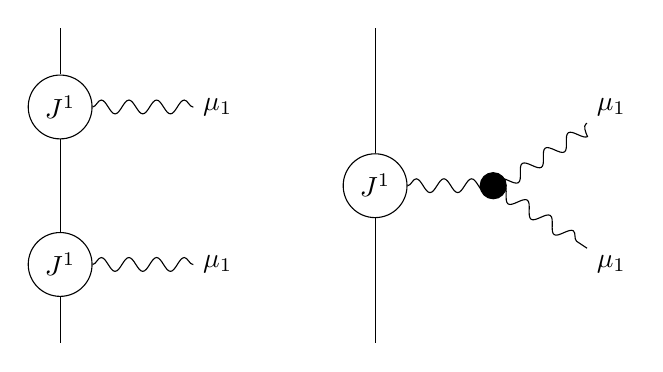
\begin{tikzpicture}
	\begin{scope}
		\node[circle, draw] (J1) at (0,1) {$\til{J}^1$};
		\node[circle, draw] (J2) at (0,-1) {$\til{J}^1$};
		\node (A1) at (2,1)  {$\mu_1$};
		\node (A2) at (2,-1)  {$\mu_1$};
		\draw[decorate, decoration={snake}] (J1) --(A1);
		\draw[decorate, decoration={snake}] (J2) --(A2);
		\draw (0,2) -- (J1) --(J2) -- (0,-2); 
	\end{scope}	
	\begin{scope}[shift={(4,0)}];
		\node[circle, draw] (J) at (0,0) {$\til{J}^1$};
		\node (A1) at (3,1)  {$\mu_1$};
		\node (A2) at (3,-1)  {$\mu_1$};
		\node[circle,draw,fill=black, minimum size = 0.2pt]  (V) at (1.5,0) {};  
		\draw[decorate, decoration={snake}] (J) -- (1.5,0) --  (A1);
		\draw[decorate, decoration={snake}] (1.5,0) --(A2);
		\draw (0,2) -- (J)-- (0,-2);
	\end{scope}
	\end{tikzpicture}
	\caption{Cancellation of the gauge anomaly of these two diagrams leads to the equation for the self OPE of the currents $\til{J}^1[k,l]$. \label{fig:JJcancel}}
\end{figure}

\subsubsection{}

Similarly, we have the $\til{J}^2 \til{J}^2$ OPE
\[ 
		\til{J}^2[r,s](0,\what{\eta}^a)  \til{J}^2[k,l](z,\what{\eta}'^{a})  
	\simeq \frac{1}{z} (l-s)  \til{J}^2 [r+k,s+l-1] (0,\what{\eta}^a + \what{\eta}'^{a} ). 
\]

the $\til{J}^1 \til{J}^2$ OPE
\[ 
	\til{J}^1[r,s] (0,\what{\eta}^a) \til{J}^2[k,l](z,\what{\eta}'^{a}) \simeq - \frac{1}{z} s  \til{J}^1[r+k, l+s - 1] (0,\what{\eta}^a + \what{\eta}'^{a})    + \frac{1}{z} k \til{J}^2[k+r-1,l+s] (0,\what{\eta}^a + \what{\eta}'^{a})  
\]
and the $\til{J}^2 \til{J}^1$ OPE
\[ 
	\til{J}^2[r,s] (0,\what{\eta}^a) \til{J}^1[k,l](z,\what{\eta}'^{a}) \simeq - \frac{1}{z} r  \til{J}^2[r+k-1, l+s ] (0,\what{\eta}^a + \what{\eta}'^{a})    + \frac{1}{z} l \til{J}^1[k+r,l+s-1] (0,\what{\eta}^a + \what{\eta}'^{a}).   
\]

\subsubsection{}

Let us use the these calculations to calculate the OPEs of the on-shell operators 
\[ 
	 	J[r,s] = r \til{J}^2[r-1,s] - s \til{J}^1[r,s-1]. 
\]
We find
\begin{multline}
	J[r,s] (0,\what{\eta}^a) J[k,l](z,\what{\eta}'^{a}) =   \frac{1}{z} (l-s) k r  \til{J}^2 [k+r-2,l+s-1]   \\
	+ \frac{1}{z} ls(k-r) \til{J}^1[k+r-1, l+s-2] \\
	+  \frac{1}{z} r (r-1) l  \til{J}^2[r+k-2, l+s -1 ]    - \frac{1}{z} l (l-1) r \til{J}^1[k+r-1,l+s-2]  \\
	+ \frac{1}{z} k s(s-1)  \til{J}^1[r+k-1, l+s - 2]    - \frac{1}{z}k s  (k-1) \til{J}^2[k+r-2,l+s-1] 
\end{multline}
(On the right hand side, all operators are evaluated at $z = 0$ and with the fermionic variables $\what{\eta}^a+\what{\eta}'^{a}$.  We have dropped this dependence for clarity.)

Collecting the terms, we find the OPE is
\begin{align*} 
	&\frac{1}{z} \left( (l-s)kr + r (r-1) l - ks (k-1)     \right)  \til{J}^2 [k+r - 2, l +s - 1]  \\
	&+ \frac{1}{z} \left( ls (k-r) - l (l-1) r + k s (s-1)  \right) \til{J}^1 [ k + r -1, l + s - 2]. 
\end{align*}

Since 
\[ 
	 J[k+r-1,l+s-1] = (k+r-1)\til{J}^2 [k+r-2,l+s-1] - (l+s-1) \til{J}^1 [ k+r - 1, l +s - 2] 
\]
we find that the OPE is 
\[ 
	J[r,s](0,\what{\eta}^a)J[k,l](z,\what{\eta}'^{a}) = \frac{1}{z} (rl-ks)  J[r+k-1,l+s-1](z, \what{\eta}^a + \what{\eta}'^{a}).     
\]

Note that the operators with $r + s = 2$ which are independent of $\what{\eta}^a$ satisfy the OPE of the $\mf{su}(2)$ Kac-Moody algebra at level \underline{zero}.
We will get a nontrivial level once we include the contribution from the back reaction, which we do in \S \ref{sec:br}. 

As was pointed out in \cite{CP}, the mode algebra corresponding to this full collection of OPE's can be expressed as the super loop space of the Lie algebra $\fw_{\infty}$ of Hamiltonoian vector fields on $\C^2$.\footnote{This is the quotient of the Lie algebra of functions on $\C^2$, which equipped with the standard Poisson bracket, by its center consisting of the constant functions.}
This is the Lie algebra $\cL^{1|4} \fw_\infty$.
Explicitly, elements of this super Lie algebra can be expressed as 
\beqn
z^{n} f(w_1,w_2; \eta_a) \in \cL^{1|4} \fw_\infty
\eeqn
for $n \in \Z$ and where $f(w_1,w_2;\eta_a) \in \C[w_1,w_2,\eta_a]/ \C$. 
The bracket is 
\beqn
[z^n f, z^m g] = z^{n+m} \eps^{ij} \del_{w_i} f \del_{w_j}g .
\eeqn

\subsection{$TJ$ OPE}

We turn to the tree-level OPE between the on-shell operators $T$ and $J$. 
First, we compute the tree-level OPE between the off-shell operators $\til{J}$ and $\til{T}$. 

The coefficient of $\til{J}^1$, for instance, in this OPE will be determined by the terms in the BRST variation of $\mu_1$ which involve $\fc_1$ and $\mu_z$ or $\fc_z$ and $\mu_1$. 
We collect such terms in the gauge variation of \eqref{eqn:j1vary} and 
\begin{equation}\label{eqn:Tvary}
\int_{(z,\eta_a) \in \C^{1|4}} \til{T} [m,n] (z,\eta_a) D_{m,n} \mu_z(z, w_i=0, \eta_a) .
\end{equation}
Recall that the gauge variation of $\mu_z$ is
\begin{align*}
Q \mu_z & = \dbar \fc_z + \mu_i \partial_{w_i} \fc_z + \mu_z \partial \fc_z - \fc_i \partial_{w_i} \mu_z - \fc_z \partial_z \mu_z \\
& -\epsilon_{ij} \partial_i \fc_\gamma \partial_j \alpha - \epsilon_{ij} \partial_i \fc_\alpha \partial_j \gamma .
\end{align*}
For now, we can disregard the terms involving $\alpha$ and $\fc_\gamma$ or $\fc_\alpha$ and $\gamma$.

The terms in the variations of \eqref{eqn:j1vary} and \eqref{eqn:Tvary} involving $\fc_1$ and $\mu_z$ or $\fc_z$ and $\mu_1$ is
\begin{align*}
& \int_{z, \eta} \til{J}^1[m,n](z,\eta_a) D_{m,n} (\mu_z \partial_{z} \fc_1 - \fc_z \partial_z \mu_1) (z, w_i=0,\eta_a) \\
+ & \int_{z,\eta} \til{T} [m,n](z,\eta_a) D_{m,n}(\mu_1 \partial_{w_1} \fc_z - \fc_1 \partial_{w_1} \mu_z) (z, w_i=0, \eta_a).
\end{align*}
The coefficient of $\fc_z$ can only be cancelled by a gauge variation of 
\[
\int_{z,z',\eta_a,\eta_a'} \til{J}^1 [r,s] (z,\eta_a) D_{r,s} \mu_1(z,w_i=0,\eta_a) \til{T} [k,l] (z',\eta_a') D_{k,l} \mu_z(z',w_i'=0,\eta_a') .
\]
By similar manipulation as above, we find that the gauge variation of this expression is 
\begin{align*}
& \int_{z,z',\eta_a,\eta_a'} \dbar_{z} \left(\til{J}^1 [r,s] (z,\eta_a) \til{T}[k,l](z',\eta_a')\right) D_{r,s} \fc_1 (z,w_i=0,\eta_a) D_{k,l} \mu_z (z',w'_i=0,\eta_a') \\
+ & \int_{z,z',\eta_a,\eta_a'} \dbar_{z'} \left(\til{J}^1 [r,s] (z,\eta_a) \til{T}[k,l](z',\eta_a')\right) D_{r,s} \mu_1 (z,w_i=0,\eta_a) D_{k,l} \fc_z (z',w'_i=0,\eta_a').
\end{align*}

To constrain the OPEs, we use the test functions $\mu_z = 0$, $\fc_1 = 0$, $\mu_1 = G(z,\zbar,\eta_a) \d \zbar w_1^k w_2^l$, 
$\fc_z = H(z,\zbar,\eta_a) w_1^r w_2^s$
for $G,H$ arbitrary smooth functions of the variables $z,\zbar,\eta_a$.
This yields the anomaly cancellation condition
\begin{multline}
\int_{z,z',\eta_a,\eta_a'} \dbar_{z'}\left(\til{J}^1 [r,s] (z,\eta_a) \til{T}[k,l](z',\eta_a')\right) G(z,\zbar,\eta_a) H(z',\zbar', \eta_a') = \\
- \int_{z'', \eta_a''} \til{J}^1[r+k, s+l] (z'', \eta_a'') H(z'', \zbar'', \eta_a'') \partial_{z''} G(z'', \zbar'', \eta_a'') \\ 
+ r \int_{z'',\eta_a''} \til{T}[r+k-1, s+l] (z'',\eta_a'') G(z'',\zbar'', \eta_a'') H(z'',\zbar'', \eta_a'') .
\end{multline}
Integrating the right hand side by parts gives us
\begin{multline}
\int_{z'', \eta_a''} \partial_{z''} \til{J}^1[r+k, s+l] (z'', \eta_a'') H(z'', \zbar'', \eta_a'') G(z'', \zbar'', \eta_a'') \\ +  \int_{z'', \eta_a''} \til{J}^1[r+k, s+l] (z'', \eta_a'') \partial_{z''} H(z'', \zbar'', \eta_a'')  G(z'', \zbar'', \eta_a'') \\
+ r \int_{z'',\eta_a''} \til{T}[r+k-1, s+l] (z'',\eta_a'') G(z'',\zbar'', \eta_a'') H(z'',\zbar'', \eta_a'') 
\end{multline}

Because $G,H$ are arbitrary functions, we arrive at the OPE
\begin{multline}
\til{T}[r,s](0,\eta_a) \til{J}^1[k,l] (z,\eta_a') \simeq \delta_{\eta_a=\eta_a'} \frac1z \partial_z \til{J}^1[r+k,s+l](0,\eta_a) + \delta_{\eta_a=\eta_a'} \frac{1}{z^2} \til{J}^1[r+k,s+l](0,\eta_a) \\ + r \delta_{\eta_a=\eta_a'} \til{T}[r+k-1,s+l] (0,\eta_a).
\end{multline}
Switching the $\eta_a$ variables to $\what{\eta}^a$ variables by applying the odd Fourier transform we can write this OPE as
\begin{multline}
\til{T}[r,s](0,\what{\eta}^a) \til{J}^1[k,l] (z,\what{\eta}'^a) \simeq \frac1z \partial_z \til{J}^1[r+k,s+l](0,\what{\eta}^a + \what{\eta}'^a) + \frac{1}{z^2} \til{J}^1[r+k,s+l](0,\what{\eta}^a + \what{\eta}'^a)  \\ + r \til{T}[r+k-1,s+l] (0,\what{\eta}^a + \what{\eta}'^a) .
\end{multline}

\subsubsection{}

In a completely similar way one can deduce the $\til{T} \til{J}^2$ OPE
\begin{multline}
\til{T}[r,s](0,\what{\eta}^a) \til{J}^2[k,l] (z,\what{\eta}'^a) \simeq \frac1z \partial_z \til{J}^2[r+k,s+l](0,\what{\eta}^a + \what{\eta}'^a) + \frac{1}{z^2} \til{J}^2[r+k,s+l](0,\what{\eta_a} + \what{\eta_a}')  \\ + s \til{T}[r+k,s+l-1] (0,\what{\eta}^a + \what{\eta}'^a) .
\end{multline}

\subsubsection{}

Using the $\til{T} \til{J}^i$ and $\til{J}^i \til{J}^2$ OPE's that we have computed, we deduce the OPE's between the on-shell operators $T$ and $J^i$. 
Recall that
\begin{equation} 
	\begin{split}
		T[r,s] &:=  \til{T}[r,s] - \frac{1}{2(r+1)} \partial_z \til{J}^1[r+1,s] - \frac{1}{2(s+1)} \partial_z \til{J}^2[r,s+1] \\
		J[k,l] &:= k \til{J}^2[k-1,l] - l \til{J}^1[k,l-1] 
	\end{split}
\end{equation}
Thus
\begin{multline}
T[r,s](0, \eta_a) J[k,l](z,\what\eta'^a) \simeq \\ k \til{T}[r,s](0, \eta_a) \til{J}^2[k-1,l] - l \til{T}[k,l](0, \eta_a) \til{J}^1[k,l-1]  \\
- \frac{k}{2(r+1)} \partial_z \til{J}^1[r+1,s] (0,\eta_a) \til{J}^2[k-1,l] + \frac{l}{2(r+1)} \partial_z \til{J}^1[r+1,s] \til{J}^1[k,l-1] \\
- \frac{k}{2(s+1)} \partial_z \til{J}^2[r+1,s] (0,\eta_a) \til{J}^2[k-1,l] + \frac{l}{2(s+1)} \partial_z \til{J}^2[r+1,s] \til{J}^1[k,l-1] .
\end{multline}
(On the right hand side, all operators are evaluated at $z = 0$ and with the fermionic variables $\what{\eta}^a+\what{\eta}'^{a}$.  We have dropped this dependence for clarity.)

\subsection{$TT$ OPE}
\label{sec:TT1}

Following the same logic we constrain the $\til{T}\til{T}$ OPE. 
These OPE's are determined by terms in the BRST variation of $\mu_z$ which involve $c_z$ and $\mu_z$. 

Proceeding as above we set
\begin{align*}
\mu_z & = G(z,\zbar,\eta_a) \d \zbar w_1^k w_2^l \\
\mf{c}_1 & = H(z,\zbar,\eta_a) w_1^r w_2^s
\end{align*}
to arrive at the anomaly constraint
\begin{multline}
\int_{z,z',\eta_a,\eta_a'} \dbar_{z'} \left(\til{T}[r,s](z,\eta_a) \til{T}[k,l](z',\eta_a') \right) G(z,\zbar,\eta_a) H(z',\zbar',\eta_a') \\
= \int_{z'',\eta''_a} \til{T} [r+k, s+l]  (z'', \eta_a'') \left(G(z'',\zbar'', \eta_a'') \partial_{z''} H(z'', \zbar'', \eta_a'') - H(z'', \zbar'', \eta_a'') \partial_{z''} G(z'',\zbar'', \eta_a'') \right) 
\end{multline}

Integrating by parts and switching to the Fourier dual odd coordinates, we find the OPE 
\begin{equation}\label{ope:TT}
\til{T}[r,s] (0,\what\eta^a) \til{T}[k,l] (z, \what\eta'^a) \simeq \frac1z \partial_z \til{T}[r+k, s+l]  (0,\what\eta^a + \what\eta'^a) + 2 \frac{1}{z^2} \til{T}[r+k, s+l]  (0,\what\eta^a + \what\eta'^a) .
\end{equation}

\subsection{$GG$ OPE}
To constrain the $G_\alpha$, $G_\gamma$ OPE we consider terms in the gauge variations of the classical couplings involving $\alpha$ and $\fc_\gamma$ or $\gamma$ and $\fc_\alpha$ (we have disregarded those terms in the analysis above as they played no role in the previous OPE calculations).

The term in the gauge variation of $\mu_i$ involving the fields $\alpha$ and $\fc_\gamma$ is $\epsilon_{ij} \partial_j \fc_\gamma \partial_z \alpha - \epsilon_{ij} \partial_z \fc_\gamma \partial_j \alpha.$
Therefore, the gauge variation of $\int \til{J}^i [m,n] D_{m,n} \mu_i$ involving such terms is
\[
\int \til{J}^i [m,n] D_{m,n} \left( \epsilon_{ij} \partial_{w_j} \fc_\gamma \partial_z \alpha - \epsilon_{ij} \partial_z \fc_\gamma \partial_{w_j} \alpha \right) .
\]
%It will be useful to integrate by parts to write this expression as
%\begin{align*}
%& \int \til{J}^i [m,n] D_{m,n} \left(-\epsilon_{ij} (\partial_{w_j} \partial_z \fc_\gamma) \alpha - \epsilon_{ij} \partial_z \fc_\gamma \partial_{w_j} \alpha \right) \\
%& + \int \epsilon_{ij} \partial_{z} \til{J}^i [m,n] D_{m,n} \partial_{w_j} \fc_\gamma \alpha 
%\end{align*}
%so that all $z$-derivatives act on $\fc_\gamma$ or $\til{J}[m,n]$. 

The term in the gauge variation of $\mu_z$ involving $\alpha$ and $\fc_\gamma$ is $-\epsilon_{ij} \partial_{w_i} \fc_\gamma \partial_{w_j} \alpha.$
Therefore, the gauge variation of $\int \til{T}[m,n] D_{m,n} \mu_z$ involving such terms is
\[
\int \til{T}[m,n] D_{m,n} (- \epsilon_{ij} \partial_{w_i} \fc_\gamma \partial_{w_j} \alpha) .
\]

The sum of these anomalies can only be cancelled by a gauge variation of a term of the form
\[
\int_{z,z',\eta_a,\eta_a'} G_\alpha[r,s] (z,\eta_a) D_{r,s} \alpha(z,w_i=0,\eta_a) G_\gamma[k,l] (z',\eta_a') D_{k,l} \gamma (z',w_i'=0,\eta_a') .
\]
The gauge variation of this expression involving the terms $\fc_\gamma$ and $\alpha$ is
\[
\int_{z,z',\eta_a,\eta_a'} \dbar_{z'} \left(G_\alpha[r,s] (z,\eta_a) G_\gamma[k,l] (z',\eta_a')\right) D_{r,s} \alpha(z,w_i=0,\eta_a) D_{k,l} \fc_\gamma (z',w_i'=0,\eta_a) .
\]

Let us plug in test fields $\alpha = \d \zbar w_1^r w_2^s G(z,\zbar,\eta_a)$ and $\fc_\gamma = w_1^k w_2^l H(z,\zbar, \eta_a)$ where $G,H$ are arbitrary functions.  
Cancellation of these gauge anomalies requires
\begin{multline}
\int_{z,z',\eta_a,\eta_a'} \dbar_{z'} \left(G_\alpha[r,s] (z,\eta_a) G_\gamma[k,l] (z',\eta_a')\right) G(z,\zbar, \eta_a) H(z',\zbar',\eta_a') = \\ l \int_{z'',\eta_a''} \til{J}^1[r+k,s+l-1] (z'',\eta_a'') H(z'',\zbar'', \eta_a'') \partial_{z''} G(z'', \zbar'', \eta_a'') \\
- k \int_{z'',\eta_a''} \til{J}^2[r+k-1,s+l] (z'',\eta_a'') H(z'',\zbar'', \eta_a'') \partial_{z''} G(z'', \zbar'', \eta_a'') \\
-s \int_{z'',\eta_a''} \til{J}^1[r+k,s+l-1] (z'',\eta_a'') \partial_{z''} H(z'',\zbar'', \eta_a'')  G(z'', \zbar'', \eta_a'') \\
+ r \int_{z'',\eta_a''} \til{J}^2[r+k-1,s+l] (z'',\eta_a'') \partial_{z''} H(z'',\zbar'', \eta_a'') G(z'', \zbar'', \eta_a'') \\
- \int_{z'',\eta_a''} \til{T}[r+k-1,s+l-1] (z'',\eta_a'') H(z'',\zbar'',\eta_a'') G(z'',\zbar'', \eta_a'') .
\end{multline}
We integrate by parts to rewrite the right hand side as
%\begin{multline}
%-l \int_{z'',\eta_a''} \partial_{z''} \til{J}^1[r+k,s+l-1] (z'',\eta_a'') H(z'',\zbar'', \eta_a'') G(z'', \zbar'', \eta_a'') \\ - l \int_{z'',\eta_a''} \til{J}^1[r+k,s+l-1] (z'',\eta_a'') \partial_{z''} H(z'',\zbar'', \eta_a'') G(z'', \zbar'', \eta_a'') \\
%+ k \int_{z'',\eta_a''} \partial_{z''}\til{J}^2[r+k-1,s+l] (z'',\eta_a'') H(z'',\zbar'', \eta_a'') G(z'', \zbar'', \eta_a'') 
%\\
%+ k \int_{z'',\eta_a''} \til{J}^2[r+k-1,s+l] (z'',\eta_a'') \partial_{z''} H(z'',\zbar'', \eta_a'') G(z'', \zbar'', \eta_a'') 
%\\
%-s \int_{z'',\eta_a''} \til{J}^1[r+k,s+l-1] (z'',\eta_a'') \partial_{z''} H(z'',\zbar'', \eta_a'')  G(z'', \zbar'', \eta_a'') \\
%+ r \int_{z'',\eta_a''} \til{J}^2[r+k-1,s+l] (z'',\eta_a'') \partial_{z''} H(z'',\zbar'', \eta_a'') G(z'', \zbar'', \eta_a'') \\
%- \int_{z'',\eta_a''} \til{T}[r+k-1,s+l-1] (z'',\eta_a'') H(z'',\zbar'',\eta_a'') G(z'',\zbar'', \eta_a'') .
%\end{multline}
\begin{multline}
\int_{z'',\eta_a''} \bigg( -l \partial_{z''} \til{J}^1[r+k,s+l-1] + k \partial_{z''} J[r+k-1,s+l] \\  - \til{T}[r+k-1, s+l-1]\bigg) (z'',\eta_a'') H(z'',\zbar'', \eta_a'') G(z'', \zbar'', \eta_a'') \\ - (s+l) \int_{z'',\eta_a''} \til{J}^1[r+k,s+l-1] (z'',\eta_a'') \partial_{z''} H(z'',\zbar'', \eta_a'') G(z'', \zbar'', \eta_a'')
\\
+ (r+k) \int_{z'',\eta_a''} \til{J}^2[r+k-1,s+l] (z'',\eta_a'') \partial_{z''} H(z'',\zbar'', \eta_a'') G(z'', \zbar'', \eta_a'') .
\end{multline}



From these expressions we can read off the OPE's just as above. 
We obtain
\begin{multline}
G_{\alpha} [r,s] (0,\what\eta_a) G_{\gamma}[k,l](z,\what\eta_a') \simeq  - (s+l) \frac{1}{z^2} \til{J}^1[r+k, s+k-1] + (r + k) \frac1{z^2} \til{J}^2 [r+k-1, s+l] \\
- l \frac1z \partial_z \til{J}^1[r+k, s+l-1] + k \frac1z\partial_z \til{J}^2 [r+k-1, s+l]
+(rl-sk) \frac1z \til{T}[r+k-1, s+l-1] .
\end{multline}
(On the right hand side, all operators are evaluated at $z = 0$ and with the fermionic variables $\what{\eta}^a+\what{\eta}'^{a}$.  We have dropped this dependence for clarity.)

\subsection{$TG$ OPE}

\end{document}
